\documentclass[12pt,dvipdfmx]{article}
\usepackage[margin=1.0truein]{geometry}
\usepackage{ifdraft}
\usepackage{subfiles}

% Math
\usepackage{amsmath}
\usepackage{amssymb}
\usepackage{bm}
\usepackage{mathrsfs}
\usepackage{mathtools}
\usepackage{optidef}
\usepackage{physics}
% https://qiita.com/rityo_masu/items/efd44bc8f9229e014237
\allowdisplaybreaks[4]
\DeclarePairedDelimiter{\floor}{\lfloor}{\rfloor}
\DeclarePairedDelimiter{\ceil}{\lceil}{\rceil}
% https://tex.stackexchange.com/questions/28836/typesetting-the-define-equals-symbol
% https://tex.stackexchange.com/questions/5502/how-to-get-a-mid-binary-relation-that-grows
\newcommand{\relmiddle}[1]{\mathrel{}\middle#1\mathrel{}}

% Theorem environments
\usepackage{amsthm}
\usepackage{thm-restate}
\theoremstyle{plain}
\newtheorem{theorem}{Theorem}
\newtheorem{proposition}{Proposition}
\newtheorem{lemma}{Lemma}
\newtheorem{assumption}{Assumption}
\newtheorem{condition}{Condition}
\newtheorem{corollary}{Corollary}

% Figure, Table, Algorithm
\usepackage{graphicx}
\usepackage{booktabs}
\usepackage{multirow}
\usepackage{makecell}
% \usepackage{mathptmx}
\usepackage{subcaption}
\usepackage{float}
\usepackage{tikz}
\definecolor{cA}{HTML}{0072BD}
\definecolor{cB}{HTML}{EDB120}
\definecolor{cC}{HTML}{77AC30}
\definecolor{cD}{HTML}{D95319}
\newcommand{\red}[1]{\textcolor{red}{#1}}
\newcommand{\blue}[1]{\textcolor{blue}{#1}}
\newcommand{\cyan}[1]{\textcolor{cyan}{#1}}
\newcommand{\gray}[1]{\textcolor{gray}{#1}}
\newcommand{\green}[1]{\textcolor{green}{#1}}
\newcommand{\brown}[1]{\textcolor{brown}{#1}}
\newcommand{\black}[1]{\textcolor{black}{#1}}
\newcommand{\orange}[1]{\textcolor{orange}{#1}}

% References
\usepackage{hyperref}
\usepackage{cleveref}
% cleveref fails to accurately capture pseudo-code line numbers. We define a custom reference command for lines in algorithms.
\crefname{assumption}{Assumption}{Assumptions}
\newcommand{\refLine}[1]{Line~\ref{#1}}
\newcommand{\refLines}[2]{Lines~\ref{#1} and \ref{#2}}

% Other packages
\usepackage{appendix}
\usepackage{cancel}
\usepackage{enumitem}
\usepackage{fancybox}
\usepackage{ifthen}
\usepackage{lipsum}
\usepackage{pifont}
\usepackage{xparse}
\usepackage{subfiles}

% https://www.reddit.com/r/LaTeX/comments/111e7gn/can_someone_help_me_replicate_these_boxes_in_latex/
\usepackage{tcolorbox}
\tcbuselibrary{skins, breakable}
\NewTotalTColorBox[auto counter]{\bookBox}{ +m +m }{
    notitle,
    colback=white,
    frame hidden,
    boxrule=0pt,
    enhanced,
    sharp corners,
    borderline west={4pt}{0pt}{cA},
    breakable,
}{
    \textcolor{cA}{
        \sffamily\textbf{#1}
    }#2
}
\NewTotalTColorBox[auto counter]{\myBox}{ +m +m }{
    notitle,
    colback=white,
    frame hidden,
    boxrule=0pt,
    enhanced,
    sharp corners,
    borderline west={4pt}{0pt}{cC},
    breakable,
}{
    \textcolor{cC}{
        \sffamily\textbf{#1}
    }#2
}

\begin{document}

\title{Supplemental Material for 04/15\\Book Reading Seminar}
\author{Hiroki Hamaguchi}
\date{2026/04/15}
\maketitle

\begin{abstract}
    \begin{center}
        This is the supplemental material for the book reading seminar.

        Please refer to the textbook and the whiteboard for the main content.

        If necessary, please also refer to my \href{https://github.com/hari64boli64/BookReadingSeminarMaterials}{repository}.
    \end{center}
\end{abstract}

\renewcommand{\theequation}{3.\arabic{equation}}
\newcommand{\setEqN}[1]{\setcounter{equation}{\numexpr#1-1\relax}}

\myBox{About the textbook}{
    \begin{figure}[H]
        \begin{minipage}{0.5\columnwidth}
            \centering
            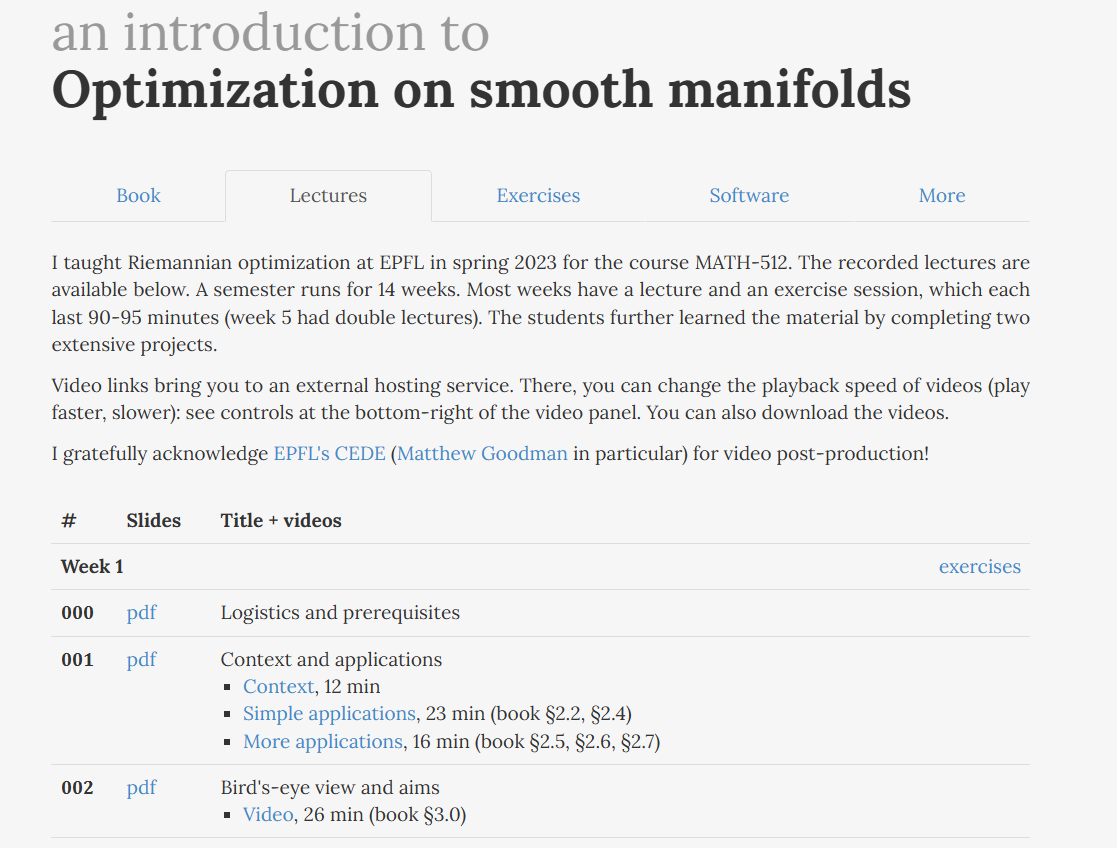
\includegraphics[width=60mm]{lectures.png}
        \end{minipage}%
        \begin{minipage}{0.5\columnwidth}
            \centering
            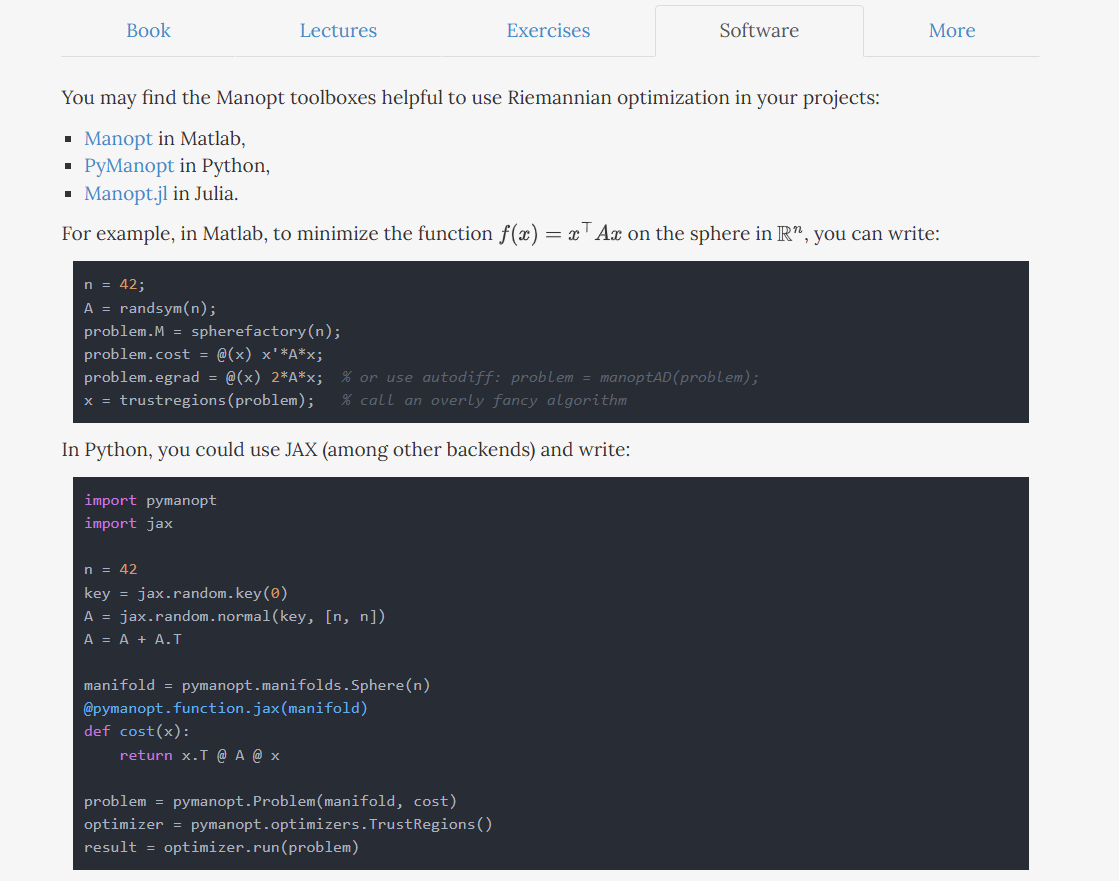
\includegraphics[width=60mm]{software.png}
        \end{minipage}
    \end{figure}
    There are lectures and software (Manopt) related to the textbook. They might be useful for understanding the textbook and doing exercises.
}
\href{https://www.nicolasboumal.net/book/#lectures}{Lectures} \href{https://www.manopt.org/}{Manopt}

\bookBox{Our goal}{
    \begin{equation}
        \min_{x \in \mathcal{M}} f(x)
    \end{equation}
}

\bookBox{Unit sphere}{
    \begin{equation}
        \mathrm{S}^{d-1} \coloneq \{ x \in \mathbb{R}^d : x^\top x = 1 \}
    \end{equation}
    \textbf{Personal Opinion:} The sphere is actually a quite good example of a manifold, but I recommend NOT to rely too much for intuition on the sphere.
}

\myBox{Smoothness}{
    \begin{equation*}
        f \text{ is smooth} \iff f \text{ is of class } C^{\infty}.
    \end{equation*}
    Adapted from Wikipedia:
    \begin{gather*}
        (U \subseteq \mathbb{R}^d \text{ is open}, \quad f\colon U \to \mathbb{R}, \quad k \in \mathbb{N})\\
        f \text{ is of class } C^k \text{ on } U\\
        \iff\\
        \forall \alpha \in \mathbb{N}^d, |\alpha| \leq k, \; \forall y \in U, \quad
        \frac{\partial^\alpha f}{\partial x_{1}^{\alpha_1} \partial x_{2}^{\alpha_2} \cdots \partial x_{d}^{\alpha_d}}(y_1, y_2, \ldots, y_d) \text{ exists and is continuous.}
    \end{gather*}
    It is known that the smoothness is also equivalent to the existence and continuity of the $k$-th Fr\'echet derivatives:
    \begin{gather*}
        (U \subseteq \mathbb{R}^d \text{ is open}, \quad f\colon U \to \mathbb{R}, \quad k \in \mathbb{N})\\
        f \text{ is of class } C^k \text{ on } U\\
        \iff\\
        \forall j \in \{1, 2, \ldots, k\}, \quad
        \forall y \in U, \quad
        \exists A \colon U \to \mathbb{R}^d, \quad \lim_{\norm{h} \to 0} \frac{\norm{f(y+h) - f(y) - A(h)}}{\norm{h}} = 0.
    \end{gather*}

    \textbf{Remark (partial differentiability vs. total differentiability):} In general, partial differentiability does not imply total differentiability (i.e., Fr\'echet differentiability). However, the above statement holds. Why? This is because the smoothness requires not only existence but also continuity of the partial derivatives. The continuity of the partial derivatives ensures that the function behaves well enough to guarantee total differentiability.\\

    \textbf{Remark (smoothness implies continuity):} If $f$ is of class $C^{\infty}$, then $f$ is of class $C^1$, and thus $f$ is continuous.
    \begin{align*}
        \lim_{y \to x} f(y) & = f(x) + \lim_{y \to x} \mathrm{D} f(x) [y-x] + \lim_{y \to x} o(\norm{y-x})                      \\
                            & \leq f(x) + \lim_{y \to x} \norm{\mathrm{D} f(x)} \cdot \norm{y-x} + \lim_{y \to x} o(\norm{y-x}) \\
                            & = f(x).
    \end{align*}
}
\href{https://en.wikipedia.org/wiki/Smoothness#Multivariate_differentiability_classes}{Wiki: Smoothness}
\href{https://en.wikipedia.org/wiki/Fr%C3%A9chet_derivative}{Wiki: Fr\'echet derivative}

\bookBox{Def 3.10}{
    \begin{gather*}
        (\mathcal{E} \text{ is a $d$-dimensional linear space}, \quad
        \emptyset \neq \mathcal{M} \subseteq \mathcal{E})\\
        \mathcal{M} \text{ is a smooth \textit{embedded submanifold} of $\mathcal{E}$ of dimension $n$}\\
        \iff\\
        \Big(n=d \text{ and } \mathcal{M} \text{ is open in } \mathcal{E} \text{ (This $\mathcal{M}$ is \textit{open submanifold})}\Big)
        \text{ or }\\
        \Big(n=d-k \; (k \geq 1) \text{ and } \forall x \in \mathcal{M}, \quad \exists U_x \subseteq \mathcal{E} \text{ is open}, \quad \exists h_x\colon U_x \to \mathbb{R}^k \text{ is smooth},\\
        (\forall y \in U_x, \quad h_x(y) = 0_k \iff y \in \mathcal{M}) \text{ and } (\mathrm{rank}(\mathrm{D} h_x(x)) = k) \Big).
    \end{gather*}
    The function $h_x$ is called a \textit{local defining function} of $\mathcal{M}$ at $x$.
}

\myBox{Notation of $U_x$}{
    In this textbook, (unlike the general definition of neighborhood) neighborhood $U$ of $x$ is defined as an open set.
    I want to explicitly indicate that it is an open and neighborhood of $x$, we use the notation ``$\exists U_x$ is open'' instaed of ``$U$'' to explicitly indicate the definition.
}

\myBox{Example: $S^2$ in $\mathbb{R}^3$}{
    \begin{equation*}
        \mathrm{S}^2 = \{ x \in \mathbb{R}^3 : x^\top x = 1 \}
        = \{ x \in \mathbb{R}^3 : h(x) = 0 \}, \quad h(x) = x^\top x - 1.
    \end{equation*}
    We can check the conditions in Def 3.10:
    \begin{gather*}
        n=2, \quad k=1, \quad d=3, \\
        h\colon U_x = \mathbb{R}^3 \subseteq \mathcal{E} = \mathbb{R}^3 \to \mathbb{R}, \quad h(x) = x^\top x - 1 \text{ is smooth},\\
        h(y) = 0 \iff y^\top y = 1 \iff y \in S^2,\\
        \mathrm{rank}(\mathrm{D} h(x)) = \mathrm{rank}(2 x^\top) = 1 \quad (\text{since } x \neq 0).
    \end{gather*}
    Thus, $\mathrm{S}^2$ is a smooth embedded submanifold of $\mathbb{R}^3$ of dimension $n=2$.
}

\myBox{Intuition of Def 3.10}{
    \begin{gather*}
        \mathrm{D} h_x(x) \simeq \mqty(\pdv{h_x}{x_1} & \cdots & \pdv{h_{x,1}}{x_d} \\ \vdots & \ddots & \vdots \\ \pdv{h_{x,k}}{x_1} & \cdots & \pdv{h_{x,k}}{x_d}) \in \mathbb{R}^{k \times d},\\
        \mathrm{rank}(\mathrm{D} h_x(x)) = k \iff \dim(\ker(\mathrm{D} h_x(x))) = d-k = n.
    \end{gather*}
    Roughly speaking, we have an $n$-dimensional (local) space in which $h_x$ is constant and thus 0 since $h_x(x) = 0$. By the definition of the local defined function $h_x$, this $n$-dimensional space is exactly $\mathcal{M} \cap U_x$. Thus, $\mathcal{M}$ is locally like an $n$-dimensional space, which is the definition of the tangent space $\mathrm{T}_x \mathcal{M}$, i.e., the dimension of $\mathcal{M}$ is $n$.

    \rule{0.98\textwidth}{0.4pt}\vspace{0.3em}

    Here is an another intuition of the definition. It seems that the definitions between the case $n=d$ and the case $n=d-k$ are different, but they are actually the same.
    \begin{gather*}
        n=d-0 \text{ and } \forall x \in \mathcal{M}, \quad \exists U_x \subseteq \mathcal{E} \text{ is open}, \quad
        \exists h_x\colon U_x \to \mathbb{R}^0=\{0\} \text{ is smooth(?)},\\
        (\forall y \in U_x, \quad h_x(y) = 0 \iff y \in \mathcal{M} \iff U_x \subseteq \mathcal{M}) \text{ and } (\mathrm{rank}(\mathrm{D} h_x(x)) = 0).
    \end{gather*}
}

\bookBox{Def 3.11}{
    The textbook's definition is somehow simplified than the general one:
    \begin{gather*}
        (\mathcal{E}_1, \mathcal{E}_2 \text{ are linear spaces},\quad U \subseteq \mathcal{E}_1, V \subseteq \mathcal{E}_2 \text{ are open})\\
        F \colon U \to V \text{ is a diffeomorphism}\\
        \iff\\
        F \text{ is a bijection and } F \text{ and } F^{-1} \text{ are smooth}.
    \end{gather*}
}
\href{https://en.wikipedia.org/wiki/Diffeomorphism}{Wiki: Diffeomorphism}

\bookBox{Theorem 3.12}{
    \begin{gather*}
        (\mathcal{E} \text{ is a $d$-dimensional linear space})\\
        \mathcal{M} \subseteq \mathcal{E} \text{ is a $n=d-k$-dimensional smooth embedded submanifold of $\mathcal{E}$}\\
        \iff\\
        \forall x \in \mathcal{M}, \quad
        \exists U_x \subseteq \mathcal{E} \text{ is open}, \quad
        \exists V \subseteq \mathbb{R}^d \text{ is open}, \\
        \exists F\colon U_x \to V \text{ is a diffeomorphism}, \\
        F(\mathcal{M} \cap U_x) = (\mathbb{R}^{n} \otimes 0_k) \cap V.
    \end{gather*}
}

\myBox{Rewrite of Theorem 3.12}{
    \begin{gather*}
        (\mathcal{E} \text{ is a $d$-dimensional linear space})\\
        \mathcal{M} \subseteq \mathcal{E} \text{ is a $n=d-k$-dimensional smooth embedded submanifold of $\mathcal{E}$}\\
        \iff\\
        \forall x \in \mathcal{M}, \quad
        \exists U_x \subseteq \mathcal{E} \text{ is open}, \quad
        \exists V \subseteq \mathbb{R}^d \text{ is open}, \\
        \exists F^{-1}\colon V \to U_x \text{ is a diffeomorphism}, \\
        F^{-1}((\mathbb{R}^{n} \otimes 0_k) \cap V) = \mathcal{M} \cap U_x.
    \end{gather*}
}

\bookBox{Non-degenerate $\mathrm{D}F^{-1}$}{
    \setEqN{20}
    \begin{equation}
        (\mathrm{D} F(x))^{-1} = D F^{-1}(F(x))
    \end{equation}
    Since $\mathrm{D} F^{-1}(F(x)) \cdot \mathrm{D} F(x) = \mathrm{D} (F^{-1} \circ F)(x) = \mathrm{D} (\mathrm{id})(x) = I_d$, this is non-degenerate.
}

\bookBox{Def 3.14}{
    \setEqN{23}
    \begin{gather}
        (\mathcal{E} \text{ is a linear space}, \quad \mathcal{M} \subseteq \mathcal{E}, \quad x \in \mathcal{M}) \notag \\
        \mathrm{T}_x \mathcal{M} \coloneq \{ c'(0) \mid
        \exists \varepsilon > 0, \quad
        \exists c\colon (-\varepsilon, \varepsilon) \to \mathcal{M} \text{ is smooth}, \quad c(0) = x \}
    \end{gather}
}

\myBox{Tangent space is a subset of the linear space}{
    \begin{equation*}
        \mathrm{T}_x \mathcal{M} \subseteq \mathcal{E}
    \end{equation*}
    This is obvious but not so trivial.
    \begin{equation*}
        c'(0) = \lim_{t \to 0} \frac{c(t) - c(0)}{t}
    \end{equation*}
    Since $c(t) \in \mathcal{M} \subseteq \mathcal{E}$ and $c(0) = x \in \mathcal{M} \subseteq \mathcal{E}$, we have $c(t) - c(0) \in \mathcal{E}$ for all $t$. Therefore, the limit is also in $\mathcal{E}$. Hence, $\mathrm{T}_x \mathcal{M} \subseteq \mathcal{E}$.

    Question: $c'(0) \in \mathcal{M}$? The answer is no. $\mathcal{M}$ is not closed under addition and scalar multiplication.
}

\bookBox{Theorem 3.15}{
    \begin{gather*}
        (\mathcal{E} \text{ is a $d$-dimensional linear space}, \quad \mathcal{M} \subseteq \mathcal{E} \text{ is}\\ \text{a smooth embedded submanifold of dimension } n, \quad x \in \mathcal{M})\\
        \begin{dcases}
            n=d                 & \implies \mathrm{T}_x \mathcal{M} = \mathcal{E}                                                       \\
            n=d-k \; (k \geq 1) & \implies \mathrm{T}_x \mathcal{M} = \ker(\mathrm{D} h_x(x)) \quad (\text{where $h_x$ is in Def 3.10})
        \end{dcases}
    \end{gather*}

    \rule{0.98\textwidth}{0.4pt}\vspace{0.3em}

    $\mathrm{T}_x \mathcal{M} \subseteq \mathcal{E}$ is already stated. We will show $\mathrm{T}_x \mathcal{M} \supseteq \mathcal{E}$.
    \vskip\baselineskip
    \textbf{Case $n=d$:} It is suffices to show that
    \begin{equation*}
        \forall v \in \mathcal{E}, \quad
        \exists \epsilon > 0, \quad
        \exists c\colon (-\epsilon, \epsilon) \to \mathcal{M} \text{ is smooth}, \quad c(0) = x, \quad c'(0) = v.
    \end{equation*}
    Since $\mathcal{M}$ is open and $x \in \mathcal{M}$, we have
    \begin{equation*}
        \exists \epsilon > 0, \quad
        \{ x + t v : t \in (-\epsilon, \epsilon) \} \subseteq \mathcal{M}.
    \end{equation*}
    Then, $c(t) \coloneq x + t v$ satisfies the required conditions.
    \vskip\baselineskip
    \textbf{Case $n=d-k$:}\\
    \textbf{Step1:} $\mathrm{T}_x \mathcal{M} \subseteq \ker(\mathrm{D} h_x \lparen x\rparen )$ % The bug of VSCode. If you write h_x (x), then the indent will break
    Recall the Def 3.10.
    \begin{gather*}
        \forall v \in \mathrm{T}_x \mathcal{M}, \quad \exists \epsilon > 0, \quad
        \exists c\colon (-\epsilon, \epsilon) \to \mathcal{M} \text{ is smooth}, \quad
        c(0) = x, \quad c'(0) = v.\\
        \forall c(t) \in U_x, \quad c(t) \in \mathcal{M} \implies h_x(c(t)) = 0_k\\
        0_k = \dv{t} h_x(c(t)) = \mathrm{D} h_x(c(t)) [c'(t)] \implies \mathrm{D} h_x(x) [v] = 0 \implies v \in \ker(\mathrm{D} h_x(x)).
    \end{gather*}
    \textbf{Step2:} $\mathrm{T}_x \mathcal{M} \supseteq (\text{$n$-dimensional subspace of } \mathcal{E})$. Recall the Theorem 3.12.
    \begin{gather*}
        \exists U_x \subseteq \mathcal{E} \text{ is open}, \quad
        \exists V \subseteq \mathbb{R}^d \text{ is open}, \\
        \exists F^{-1}\colon V \to U_x \text{ is a diffeomorphism}, \\
        F^{-1}((\mathbb{R}^{n} \otimes 0_k) \cap V) = \mathcal{M} \cap U_x.
    \end{gather*}
    We can construct a curve $c$ to use the definition of $\mathrm{T}_x \mathcal{M}$ as follows:
    \begin{gather*}
        \forall u \in \mathbb{R}^n, \quad
        \exists \epsilon > 0, \quad
        c\colon (-\epsilon, \epsilon) \to \mathbb{R}^d, \quad c(t) = F^{-1}(F(x) + t (u \otimes 0_k)) \text{ is smooth},\\
        c(0) = F^{-1}(F(x)) = x, \quad c'(0) =
        \mathrm{D} F^{-1}(F(x)) [u \otimes 0_k].
    \end{gather*}
    Thus, $\mathrm{T}_x \mathcal{M}$ contains the $n$-dimensional subspace, which is $\ker(\mathrm{D} h_x \lparen x \rparen)$.
}

\bookBox{Definition 3.16}{
    \begin{equation*}
        \dim\;\mathcal{M} \coloneq \dim \mathrm{T}_x \mathcal{M} \text{ at some } x \in \mathcal{M} \neq \emptyset.
    \end{equation*}
    This is exactly the $n$ in Definition 3.10
    (TOP IMPORTANCE IN THIS MATERIAL).
}

\myBox{The general definition of manifold}{\\
    The textbook discusses the Definition 3.16 based on Theorem 3.15, so it might seem that the definition of dimension is only applicable to embedded submanifolds. However, as can be seen from the fact that the term ``embedded submanifold'' does not appear in Definition 3.16, the dimension can actually be defined for general manifolds, and rather the dimension itself is included in the definition of a manifold. In this textbook, we do not cover the precise definition of manifolds in order to get to optimization as quickly as possible. Therefore, as a supplement, we will introduce the general definition of manifolds and the definition of dimension for general manifolds.

    \textbf{Coordinate neighborhood:}
    \begin{gather*}
        (X \text{ is a topological space}, \quad U \subseteq X \text{ is open}, \quad U' \subseteq \mathbb{R}^m \text{ is open})\\
        (U, \phi) \text{ is an $m$-dimensional coordinate neighborhood} \iff \phi\colon U \to U' \text{ is a homeomorphism}.
    \end{gather*}
    \textbf{Manifold:}
    \begin{gather*}
        (\mathcal{M} \text{ is a topological space})\\
        \mathcal{M} \text{ is a smooth topological manifold of dimension $m$}\\
        \iff\\
        \begin{dcases}
            (1) & \mathcal{M} \text{ is Hausdorff: } \forall x, y \in \mathcal{M}, x \neq y, \exists U_x, U_y \text{ are open}, U_x \cap U_y = \emptyset.                                                                      \\
            (2) & \exists \{(U_\alpha, \phi_\alpha)\}_{\alpha \in A} (\text{ $m$-dimensional coordinate neighborhoods}),\quad M=\bigcup_{\alpha \in A} U_\alpha,                                                               \\
            (3) & \forall \alpha, \beta \in A, U_\alpha \cap U_\beta \neq \emptyset, \quad \phi_\beta \circ \phi_\alpha^{-1}\colon \phi_\alpha(U_\alpha \cap U_\beta) \to \phi_\beta(U_\alpha \cap U_\beta) \text{ is smooth}.
        \end{dcases}
    \end{gather*}
}

\bookBox{Example 3.19}{
    \begin{figure}[H]
        \centering
        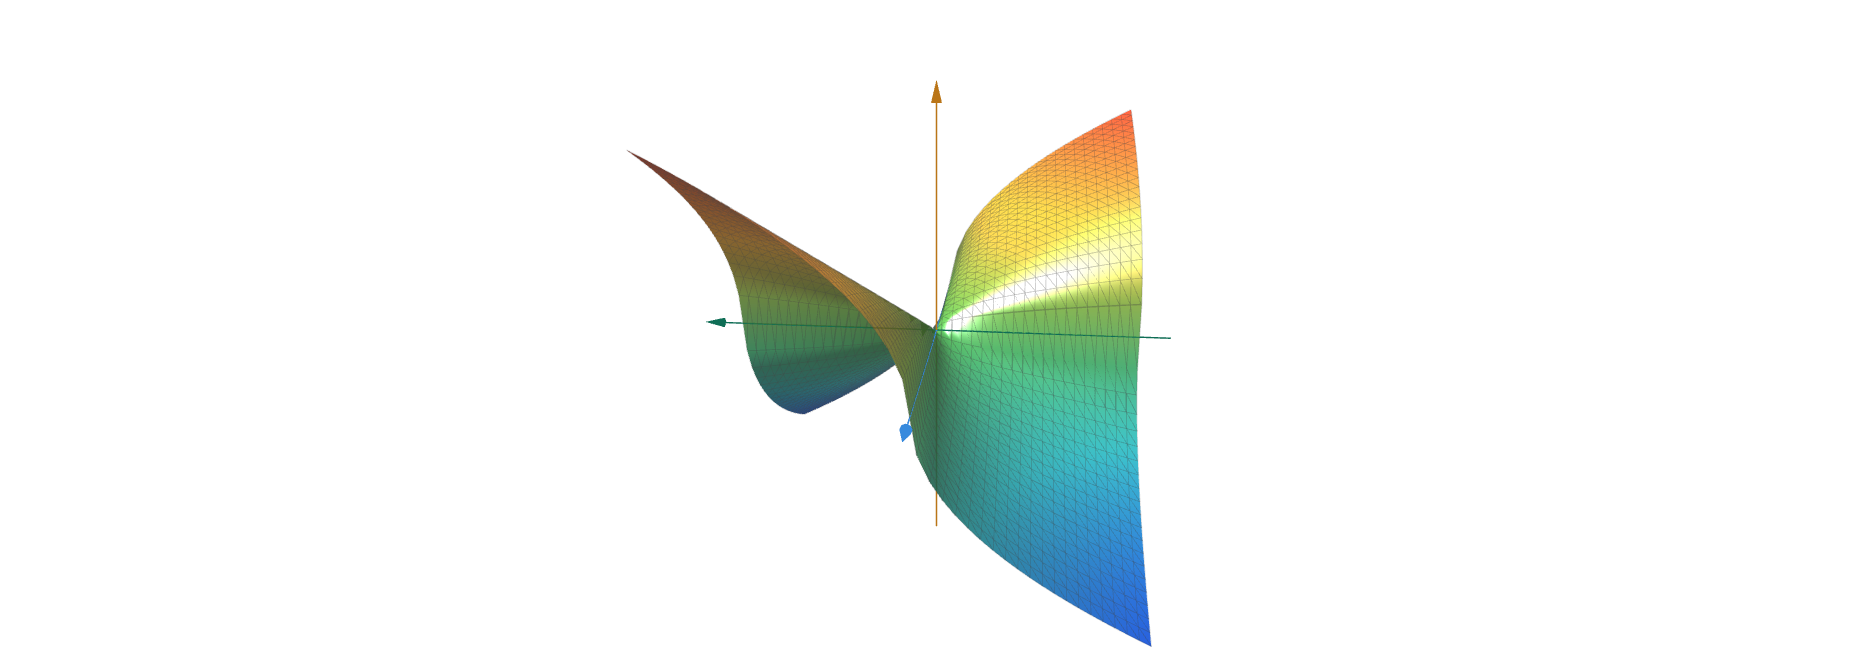
\includegraphics[height=5cm]{Sym21.png}
        \caption{Visualization of $x_1 x_3 = x_2^2$ in $\mathbb{R}^3$. The orange axis represents $x_2$.}
        \label{fig:Sym21}
    \end{figure}
    \begin{figure}[H]
        \centering
        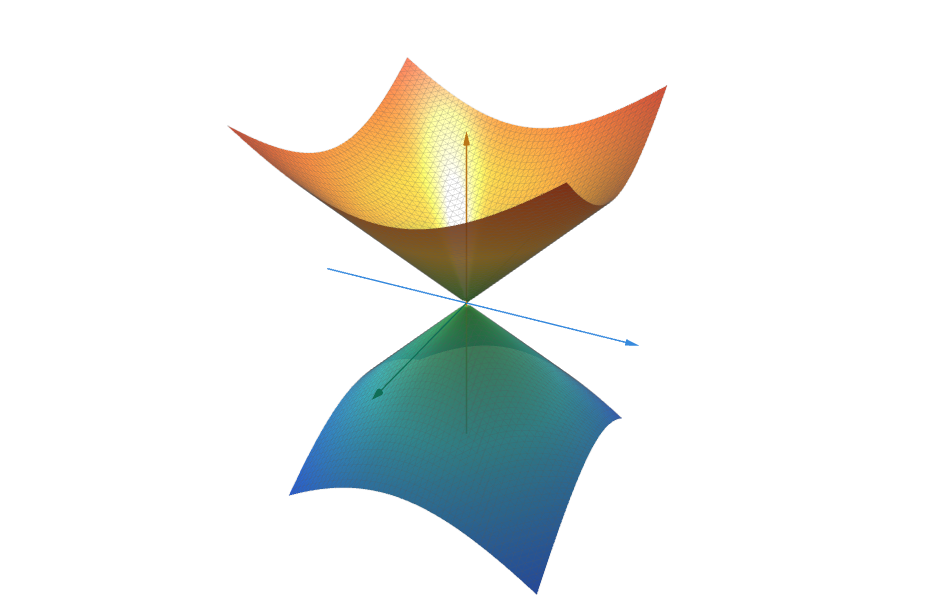
\includegraphics[height=5cm]{Sym21_cone.png}
        \caption{Visualization of $z_1^2 + z_2^2 = z_3^2$ in $\mathbb{R}^3$. The orange axis represents $z_3$.}
        \label{fig:Sym21_cone}
    \end{figure}
    We show the visualization in \cref{fig:Sym21,fig:Sym21_cone}.
}

\myBox{Proposition 3.20 and Exercise 3.25}{
    \begin{gather*}
        \Big(\mathcal{E}, \mathcal{E}' \text{ are $d,d'$-dimensional linear spaces},\\
        \mathcal{M} \subseteq \mathcal{E}, \mathcal{M}' \subseteq \mathcal{E}' \text{ are smooth embedded submanifolds} \text{ of dimension } n, n' \Big)\\
        \begin{dcases}
            \mathcal{M} \times \mathcal{M}' \text{ is a smooth embedded submanifold of } \mathcal{E} \times \mathcal{E}' \\
            \mathrm{T}_{(x, x')} (\mathcal{M} \times \mathcal{M}') = \mathrm{T}_x \mathcal{M} \times \mathrm{T}_{x'} \mathcal{M}'
        \end{dcases}
    \end{gather*}

    \rule{0.98\textwidth}{0.4pt}\vspace{0.3em}

    \textbf{First part:}\\
    \textbf{Case $n=d$ and $n'=d'$:} $\mathcal{M} \times \mathcal{M}'$ is open in $\mathcal{E} \times \mathcal{E}'$ by the definition of the product topology.

    \textbf{Case $n=d$ and $n' = d'-k'$:} omitted.

    \textbf{Case $n=d-k$ and $n' = d'-k'$:}
    \begin{gather*}
        \forall (x, x') \in \mathcal{M} \times \mathcal{M}', \quad
        \exists U_{x,x'} \coloneqq U_x \times U_{x'} \subseteq \mathcal{E} \times \mathcal{E}' \text{ is open}, \\
        \exists h_{x,x'}\colon U_{x,x'} \to \mathbb{R}^{k+k'} \text{ is smooth defined by } h_{x,x'}(y, y') = (h_x(y), h_{x'}(y')),\\
        \Biggr(\forall (y, y') \in U_{x,x'}, \quad h_{x,x'}(y, y') = 0_{k+k'} \iff (y, y') \in \mathcal{M} \times \mathcal{M}' \text{ and }\\
        \left(\mathrm{rank}(\mathrm{D} h_{x,x'}(x, x')) = \mathrm{rank}\left(\mqty(\mathrm{D} h_x(x) & 0 \\ 0 & \mathrm{D} h_{x'}(x'))\right) = k + k' \right) \Biggr).
    \end{gather*}

    \textbf{Second part:} Similar. Omitted.
}

\bookBox{Proposition 3.23 and Exercise 3.26}{
    By definition. Omitted.
}

\myBox{Lemma for Exercises 3.27--3.29}{
    \begin{equation*}
        \mathcal{M} \in \{\mathcal{X}, \mathcal{C}, \mathcal{P}\}.
    \end{equation*}
    These exercises require to prove that the manifolds provided are not an embedded submanifolds of $\mathcal{E}$.
    We can check the conditions in Def 3.10.
    Note that $\mathcal{E} = \mathbb{R}^2$ with $d=2$.

    For the sake of solving these exercises, we first prove that, if manifold $\mathcal{M} \in \{\mathcal{X}, \mathcal{C}, \mathcal{P}\}$ is an embedded submanifold of $\mathrm{R}^2$, then the dimension of the manifold $k$ must be 1.
    \vskip\baselineskip
    \textbf{Case $n=d=2$:} Since $\mathcal{M}$ is not open in $\mathbb{R}^2$, $\mathcal{M}$ is not an open submanifold. Thus, $k\neq 0$.\\
    \textbf{Case $n=d-k \; (k \geq 1)$:} Let $h$ to be the local defining function.
    Since the dimension of $\mathrm{T}_x \mathcal{M}$ is at least 1 at some $x \in \mathcal{M}$ by the figures at p.26 of the textbook (and the definition), we have $\dim \ker \mathrm{D}h(x) \geq 1$.
    By the rank-nullity theorem, we have $\mathrm{rank} \mathrm{D} h(x) \leq 1$.
    Since $\mathrm{rank} \mathrm{D} h(x) = k$ and $k \geq 1$, it follows that $k=1$.
}

\myBox{Exercise 3.27}{
    \begin{equation*}
        \mathcal{X} \coloneqq \{ x \in \mathbb{R}^2 : x_1^2 = x_2^2 \}
    \end{equation*}
    Assume that
    \begin{gather*}
        \forall x \in \mathcal{X}, \quad
        \exists U_x \subseteq \mathbb{R}^2 \text{ is open}, \quad
        \exists h_x\colon U_x \to \mathbb{R}^k \text{ is smooth},\\
        (\forall y \in U_x, \quad h_x(y) = 0_k \iff y \in \mathcal{X}) \text{ and } (\mathrm{rank}(\mathrm{D} h_x(x)) = k).
    \end{gather*}
    Consider lines $x_1=x_2$ and $x_1=-x_2$. We have $h_x(y)=0$ for any point $y$ on these lines. Thus, $\mathrm{D}h_x\lparen x \rparen \mqty[1 \\ 1] = 0$ and $\mathrm{D}h_x \lparen x \rparen \mqty[1 \\ -1] = 0$.
    This means that $\mathrm{D} h_x \lparen x \rparen$ is degenerate. However, $\mathrm{rank}(\mathrm{D} h_x \lparen x \rparen) = k \geq 1$, which is a contradiction. Thus, $\mathcal{X}$ is not a smooth embedded submanifold of $\mathbb{R}^2$.
}

\myBox{Exercise 3.28}{
    \begin{equation*}
        \mathcal{C} \coloneqq \{ x \in \mathbb{R}^2 : x_1^2 = x_2^3 \}
    \end{equation*}
    Let us compute the tangent space at the origin $0 \in \mathcal{C}$:
    \begin{equation*}
        \mathrm{T}_0 \mathcal{C} = \{ c'(0) \mid
        \exists \varepsilon > 0, \quad
        \exists c\colon (-\varepsilon, \varepsilon) \to \mathcal{C} \text{ is smooth}, \quad c(0) = 0 \}.
    \end{equation*}
    On $\mathcal{C}$, we can only approach the origin along the positive $x_2$-axis. Thus, $c'(0) = 0$, otherwise, $c$ cannot be smooth. (we can show it by contradiction.)
    Thus, $\mathrm{T}_0 \mathcal{C} = \{ 0 \}$, which is a degenerate subspace of $\mathbb{R}^2$. However, $\mathrm{rank}(\mathrm{D} h_0 \lparen 0 \rparen) = k = 1$, which is a contradiction. Thus, $\mathcal{C}$ is not a smooth embedded submanifold of $\mathbb{R}^2$.
}

\myBox{Exercise 3.29}{
    \begin{equation*}
        \mathcal{P} \coloneqq \{ x \in \mathbb{R}^2 : x_1^2 = x_2^4 \}
    \end{equation*}
    Apply Theorem 3.12 at the origin $0 \in \mathcal{P}$:
    \begin{gather*}
        \exists U_0 \subseteq \mathbb{R}^2 \text{ is open}, \quad
        \exists V \subseteq \mathbb{R}^2 \text{ is open}, \\
        \exists F^{-1}\colon V \to U_0 \text{ is a diffeomorphism}, \\
        F^{-1}((\mathbb{R}^{1} \otimes 0_1) \cap V) = \mathcal{P} \cap U_0. \quad (\bigstar)
    \end{gather*}
    Since $0 \in \mathcal{P} \cap U_0$ by definition, we have $F(0) \in (\mathbb{R}^{1} \otimes 0_1) \cap V$ by $(\bigstar)$.
    Let us define $F(0) = (a, 0)$ for some $a \in \mathbb{R}$. Since $V$ is open, there exists $\epsilon > 0$ such that $(a+t, 0) \in V$ for all $t \in (-\epsilon, \epsilon)$.
    Let us define
    \begin{equation*}
        c(t) = F^{-1}(a+t, 0) \quad (t \in (-\epsilon, \epsilon)).
    \end{equation*}
    Since $F^{-1}$ is diffeomorphism, $c$ is also diffeomorphism, i.e., bijective, invertible, and both $c$ and $c^{-1}$ are smooth.
    It is obvious that $\{(a+t, 0) : t \in (-\epsilon, \epsilon)\} \subseteq (\mathbb{R}^{1} \otimes 0_1) \cap V$. Thus, $\{c(t) : t \in (-\epsilon, \epsilon)\} \subseteq \mathcal{P} \cap U_0$ by $(\bigstar)$. Since the image of smooth (i.e., continuous) map of an interval is open, and that $c(0)= F^{-1}(a, 0) = F^{-1}(F(0)) = 0$, we have $\{c(t) : t \in (-\epsilon, \epsilon)\}$ is an open neighborhood of $0$. Thus, there exists $\delta_1, \delta_2, \delta_3, \delta_4 > 0$ such that
    \begin{align*}
        \{ (+x^2, +x) : x \in (0, \delta_1) \} & \subseteq \{c(t) : t \in (-\epsilon, \epsilon)\}  \\
        \{ (-x^2, +x) : x \in (0, \delta_2) \} & \subseteq \{c(t) : t \in (-\epsilon, \epsilon)\}  \\
        \{ (+x^2, -x) : x \in (0, \delta_3) \} & \subseteq \{c(t) : t \in (-\epsilon, \epsilon)\}  \\
        \{ (-x^2, -x) : x \in (0, \delta_4) \} & \subseteq \{c(t) : t \in (-\epsilon, \epsilon)\}.
    \end{align*}
    Thus, we have 4 distinct intervals as follows:
    \begin{align*}
        \{ c^{-1}(F((+x^2, +x))) : x \in (0, \delta_1) \} & \subseteq (-\epsilon, \epsilon)  \\
        \{ c^{-1}(F((-x^2, +x))) : x \in (0, \delta_2) \} & \subseteq (-\epsilon, \epsilon)  \\
        \{ c^{-1}(F((+x^2, -x))) : x \in (0, \delta_3) \} & \subseteq (-\epsilon, \epsilon)  \\
        \{ c^{-1}(F((-x^2, -x))) : x \in (0, \delta_4) \} & \subseteq (-\epsilon, \epsilon).
    \end{align*}
    Indeed, since $c$ is invertible and smooth (i.e., continuous), these sets are intervals in $(-\epsilon, \epsilon)$. They are also distinct since $c^{-1}$ and $F$ are bijective and the domain of $c^{-1} \circ F$ are 4 distinct set.
    We also have that an sequence in $\{ c^{-1}(F((+x^2, +x))) : x \in (0, \delta_1) \}$ converges to $0$ as $x \to 0$, and the same holds for the other 3 sets. Thus, we have 4 distinct intervals in $(-\epsilon, \epsilon)$ that converge to $0$. This is a contradiction since there are at most 2 distinct intervals in $(-\epsilon, \epsilon)$ that converge to $0$. Thus, $\mathcal{P}$ is not a smooth embedded submanifold of $\mathbb{R}^2$.
}

\bookBox{Definition 3.30}{
    \begin{gather*}
        (\mathcal{M}, \mathcal{M}' \text{ are smooth embedded submanifolds of } \mathcal{E}, \mathcal{E}' \text{ respectively}, \; x \in \mathcal{M})\\
        F \colon \mathcal{M} \to \mathcal{M}' \text{ is smooth at } x\\
        \iff\\
        ( \exists U_x \subseteq \mathcal{E} \text{ is open}, \quad
        \exists \bar{F} \colon U_x \to \mathcal{E}' \text{ is smooth}, \quad
        \bar{F}(y) = F(y) \text{ for all } y \in \mathcal{M} \cap U_x)
    \end{gather*}
    Note that the smoothness of $\bar{F}$ is already defined at the beginning of this material.
    $\bar{F}$ is called a \textit{local smooth extension} of $F$ at $x$.
    \begin{equation*}
        F \text{ is smooth} \iff \forall x \in \mathcal{M}, \quad F \text{ is smooth at } x.
    \end{equation*}
}

\bookBox{Proposition 3.31}{
    \begin{gather*}
        (\mathcal{M}, \mathcal{M}' \text{ are smooth embedded submanifolds of } \mathcal{E}, \mathcal{E}' \text{ respectively}, \; x \in \mathcal{M})\\
        F \colon \mathcal{M} \to \mathcal{M}' \text{ is smooth}\\
        \iff\\
        \exists U \subseteq \mathcal{E} \text{ is open}, \quad \mathcal{M} \subseteq U \quad
        \exists \bar{F} \colon U \to \mathcal{E}' \text{ is smooth}, \quad
        \bar{F}(y) = F(y) \text{ for all } y \in \mathcal{M}
    \end{gather*}
}

\myBox{Proof of Proposition 3.31}{\\
    \textbf{Only if part:} Difficult. We use the paracompactness of $\mathcal{M}$ and the partition of unity.
    \begin{figure}[H]
        \centering
        \includegraphics[width=\columnwidth]{partition_of_unity.png}
        \caption{Cited from Wikipedia.}
    \end{figure}
    \begin{gather*}
        \exists \{ U_{x_i} \}_{i \in I} \text{ is an finite open cover of } \mathcal{M},\\
        \exists \{ \phi_i \}_{i \in I} \text{ is a partition of unity subordinate to } \{ U_{x_i} \}_{i \in I}.
    \end{gather*}
    Then, we can construct a local smooth extension $\bar{F}$ of $F$ as follows:
    \begin{equation*}
        \bar{F}(y) = \sum_{i \in I} \phi_i(y) \bar{F}_{x_i}(y) \quad \qty(y \in U \coloneq \bigcup_{i \in I} U_{x_i}),
    \end{equation*}
    where $\bar{F}_{x_i}$ is a local smooth extension of $F$ at $x_i$.
    We can check that $\bar{F}$ is a local smooth extension of $F$ at any point $x \in \mathcal{M}$ as follows:
    \begin{equation*}
        \bar{F}(y) = \sum_{i \in I} \phi_i(y) \bar{F}_{x_i}(y) = \sum_{i \in I} \phi_i(y) F(y) = F(y) \quad (y \in \mathcal{M}).
    \end{equation*}
    The smoothness of $\bar{F}$ is trivial since it is a finite sum of products of smooth functions.
    \vskip\baselineskip
    \textbf{If part:} trivial.
}
\href{https://ja.wikipedia.org/wiki/%E3%83%91%E3%83%A9%E3%82%B3%E3%83%B3%E3%83%91%E3%82%AF%E3%83%88%E7%A9%BA%E9%96%93}{Wiki: Paracompact space}
\href{https://ja.wikipedia.org/wiki/1%E3%81%AE%E5%88%86%E5%89%B2}{Wiki: Partition of unity}

\myBox{Exercise 3.32}{
    \begin{equation*}
        \mathrm{Sym}(2)_1 \subseteq U=\mathrm{Sym}(2) \setminus \{ 0 \} \subseteq \mathcal{E} = \mathrm{Sym}(2).
    \end{equation*}
    Let $f$ be a smooth function on $U$ which is defined on $\mathcal{E}=\mathrm{Sym}(2)$ as follows:
    \begin{equation*}
        f(X) = \begin{cases}
            \frac{1}{\|X\|} & X \neq 0 \\
            0               & X = 0
        \end{cases}
    \end{equation*}
    Then, smooth extension of $f$ from $U$ to $\mathcal{E}$ doesn't exist since it cannot be smooth at $0$ by definition.
}

\myBox{Exercise 3.37}{\\
    We add a hypothesis that $\mathcal{M}$ is a smooth embedded submanifold of $\mathcal{E}$. Otherwise, the statement can be undefined in the context of this textbook.
    By Proposition 3.31, we have
    \begin{gather*}
        \exists U_1 \subseteq \mathcal{E} \text{ is open}, \; \mathcal{M} \subseteq U_1, \quad \exists \bar{F}_1 \colon U_1 \to \mathcal{E}' \text{ is smooth}, \quad \bar{F}_1(y) = F(y) \text{ for all } y \in \mathcal{M},\\
        \exists U_2 \subseteq \mathcal{E} \text{ is open}, \; \mathcal{M} \subseteq U_2, \quad \exists \bar{F}_2 \colon U_2 \to \mathcal{E}' \text{ is smooth}, \quad \bar{F}_2(y) = F(y) \text{ for all } y \in \mathcal{M}.
    \end{gather*}
    Thus, we have
    \begin{gather*}
        \mathcal{M} \subseteq U_1 \cap U_2 \subseteq \mathcal{E}, \quad \bar{F} \coloneq a_1 \bar{F}_1 + a_2 \bar{F}_2 \colon U_1 \cap U_2 \to \mathcal{E}' \text{ is smooth},\\
        \bar{F}(y) = a_1 \bar{F}_1(y) + a_2 \bar{F}_2(y) = a_1 F_1(y) + a_2 F_2(y) = F(y) \quad (y \in \mathcal{M}).
    \end{gather*}
    This means that $F$ is smooth.
    By proposition 3.35, we also have
    \begin{equation*}
        \mathrm{D} F(x) = \mathrm{D} \bar{F}(x) |_{\mathrm{T}_x \mathcal{M}} = a_1 \mathrm{D} \bar{F}_1(x) |_{\mathrm{T}_x \mathcal{M}} + a_2 \mathrm{D} \bar{F}_2(x) |_{\mathrm{T}_x \mathcal{M}} = a_1 \mathrm{D} F_1(x) + a_2 \mathrm{D} F_2(x).
    \end{equation*}
}

\myBox{Exercise 3.38, 3.39}{\\
    Almost the same as Exercise 3.37. Omitted.
}

\myBox{Exercise 3.40}{\\
    Almost the same as Exercise 3.37. We only show the case $\mathcal{M}=\mathrm{R}^{m_1}, \mathcal{M}'=\mathrm{R}^{m_2}, \mathcal{N}=\mathrm{R}^{n_1+n_2}$.
    Take an arbitrary point $(x, y) \in \mathcal{M} \times \mathcal{M}'$, and define
    \begin{equation*}
        F_1^{(x,y)}\colon \mathrm{R}^{m_1} \to \mathrm{R}^{n_1}, F_1(x') = F(x', y), \quad
        F_2^{(x,y)}\colon \mathrm{R}^{m_2} \to \mathrm{R}^{n_2}, F_2(y') = F(x, y').
    \end{equation*}
    Then, we have
    \begin{equation*}
        \mathrm{D}F(x,y)[(u,v)] = \mqty[\mathrm{D} F_1^{(x,y)}(x) & 0 \\ 0 & \mathrm{D} F_2^{(x,y)}(y)] \mqty[u \\ v] = \mathrm{D} F_1^{(x,y)}(x) u + \mathrm{D} F_2^{(x,y)}(y) v.
    \end{equation*}
}

\end{document}
